% LaTeX project: A template for MUST Thesis v0.1.0.8
%
% MUSTthesis (https://github.com/iihciyekub/must-thesis) bindings for XeLaTeX
% Author: Y.J.Li(iihciyekub)
% GitHub: https://github.com/iihciyekub/must-thesis
%
%
% Copyright 2019 Y.J.Li
%
% This work may be distributed and/or modified under the
% conditions of the LaTeX Project Public License, either version 1.3
% of this license or (at your option) any later version.
% The latest version of this license is in
%   http://www.latex-project.org/lppl.txt
% and version 1.3 or later is part of all distributions of LaTeX
% version 2005/12/01 or later.
%
% This work has the LPPL maintenance status `maintained'.
% 
% The Current Maintainer of this work is Y.J.Li
%
% This work consists of the files MUSTthesis.tex, MUSTthesisC.cls and MUSTthesiS.sty
%
%% MUSTthesis.tex - Demo for MUSTthesis %%
%% Last Modified: 2019-06-11 %%


%!TEX encoding 	= UTF-8
%!TEX program 	= xelatex
\documentclass{format/MUSTThesisC}




\begin{document}

%% -------------------------------------------------<< \readme  % MUST Thesis 模版项目说明,仅用于展示说明
																% 毕业论文正式启用时请直接删去 \input 整行语句.
%% -------------------------------------------------<< \readme 為 MUST Thesis 模版說明,正式使用時註釋掉
\newgeometry{left=0cm,right=0cm,top=0cm, bottom=0cm}
\thispagestyle{empty}
\vfill
\begin{center}
	\begin{tikzpicture}
		% 子圖全局透明設置
		\begin{scope}[opacity=0.0]
			\draw[help lines,gray!20,step=1cm] (-0.49\paperwidth,-0.49\paperheight) grid (0.49\paperwidth,0.49\paperheight);
			\fill (0,0) circle (1pt);
			\foreach \i in {-10,-9,...,10}
			\node at (\i,0) {{\large \i}};
			\foreach \i in {-14,-13,...,14}
			\node at (0,\i) {{\large \i}};
		\end{scope}

		% GitHub 下載
		\coordinate (cd1) at (-7.6,13.5);
		\node[black!80](githubico) at (cd1) {\sfz{20pt}\faGithub};
		\node[right=-2.87pt of githubico.east,fill=black!80,rectangle, rounded corners=2pt] {\url{https://github.com/iihciyekub/mustthesis}};
		\draw[white,line width=1.3pt]  (cd1) circle (10pt);



		% 校徽logo
		\path
		let \p1 =(-4,2) in
		% 節點放置校徽圖片
		node(logo)[anchor=east] at (\p1) {
\includegraphics[width=3.5cm]{figure/MUSTSchoolBadgecolor}}
		%  澳門科技大學
		node(c)[anchor=west,text width =10cm,right=1pt of logo.15]  {\sfz{35pt}澳\hfill 門\hfill 科\hfill 技\hfill 大\hfill 學}


		% 學校英文名
		node(must)[anchor=west,text width=10cm,right=1pt of logo.-15] {\color{gray}\sfz{10pt}\textbf{MACAU \hfill UNIVERSITY\hfill OF\hfill SCIENCE\hfill AND\hfill TECHNOLOGY}}
		% 線段
		node[anchor= west,right=1pt of logo.-21]{\rule{10cm}{0.7pt}}
		node[anchor= west,right=1pt of logo.-22]{\rule{2.87cm}{1.6pt}}
		% 學院
		node(SOB)[anchor=north west,right=1pt of logo.-28,gray]{{\footnotesize School of Business,2018}}
		% 版本說明
		node[left=0pt of c.east,yshift=10mm]{\color{Salmon}\footnotesize\projectBname \color{black!60} \sfz{18pt}{\faGraduationCap} }


		node(L1)[anchor= north west,white,text height=5pt,fill=black!80,rectangle, rounded corners=1pt,right=2pt of logo.-37]
			{\href{https://www.latex-project.org/lppl/}{ \color{white}\sfz{7pt}\texttt{\rlap{\color{black!80}p}Licenes:}}}
		node(L2)[anchor= north west,text height=5pt,right = 0mm of L1,rectangle, fill=Periwinkle!80,rounded corners=1pt,right=1pt of L1] {\href{https://www.latex-project.org/lppl.txt}{\color{white}\sfz{7pt}\texttt{The LaTeX Project Public License (LPPL v1.3c)}}}
		node[anchor=north west,right=0pt of L2]{\faBalanceScale\faCreativeCommons}
		;





		% author 作者信息	
		\begin{scope}
			\tikzstyle{a}=[draw=black!40,line width=1.5pt]
			\coordinate (P1) at (5,-11);
			\clip (P1) circle (0.55cm);
			\node(note2) at (P1) {\includegraphics[width=1.2cm]{figure/author}};
			\draw[a]  (P1) circle (0.55cm);
		\end{scope}


		\node(e)[right=-1mm of note2.east,yshift=2mm] {};
		\node(ee2)[right=-1mm of note2.east,yshift=-12mm] {};
		\draw[Goldenrod,line width=3pt,name=l1] (e)--(ee2);

		\node(name1)[right=-.5mm of e ,anchor=north west] {\href{mailto:lyj8512@126.com}{\texttt{@}\iiname}};
		\node[right=-.5mm of name1.west,yshift=-1.2em,gray] {\color{LimeGreen}{\faWechat} \color{gray}\texttt{iichieykub}};
		\node[right=-.5mm of name1.west,yshift=-2.4em,gray] {{\footnotesize \texttt{Copyright} \copyright  \texttt{2019}}\iiname};

	\end{tikzpicture}
\end{center}

\vfill


%% 第二頁
\newpage
\thispagestyle{empty}

\vfill
\begin{center}
	\begin{tikzpicture}

		%% -------------------------------------------------<< 子圖全局透明設置
		\begin{scope}[opacity=0]
			\draw[help lines,gray!20,step=1cm] (-0.49\paperwidth,-0.49\paperheight) grid (0.49\paperwidth,0.49\paperheight);
			\fill (0,0) circle (1pt);
			\foreach \i in {-10,-9,...,10}
			\node at (\i,0) {{\large \i}};
			\foreach \i in {-14,-13,...,14}
			\node at (0,\i) {{\large \i}};
		\end{scope}




		%% -------------------------------------------------<<
		% 設置版本節點的樣式
		\tikzset{gitnode/.style={anchor=east,fill=#1!50, draw=#1, text=black,rounded corners=2pt,opacity=0.7,node font=\texttt,font=\large,line width=0.6pt}}
		\tikzset{gitsubnode/.style={anchor=east,fill=#1!50, circle=1pt,draw=#1, text=black!60,line width=0.6pt}}

		% 設置全局坐標點
		\coordinate (git1) at (-5.5,12.5);
		\filldraw[gray!10!blue!2!red!1,opacity=0.2,rounded corners=5pt,draw=black,line width=.8pt,name path=A]
		let \p1=(git1) in
		(\x1-4cm,\y1+1.1cm) rectangle +(19.2cm,-5.78) ;

		% 發佈版本節點的代碼
		\node(m1)[gitnode=LimeGreen] at (git1){\texttt{Release}};
		\draw[dashed,line width=.8pt,gray!40]   ($(m1.east)+(3mm,0)$) -- +(2cm,0)node[gitsubnode=LimeGreen,name=mm1]{}
		--+(4.7cm,0)node[gitsubnode=LimeGreen,name=v2]{}
		--+(12.4cm,0)node[gitsubnode=LimeGreen,name=v3]{}
		+(13,0);

		% v0.0.0.1
		\node[anchor=east,right=-6pt of mm1.west,yshift=5mm]  at (mm1) {\faHandODown\texttt{~v0.0.0.1}};
		% v0.0.0.4
		\node[anchor=east,right=-6pt of v2.west,yshift=5mm]  at (v2) {\faHandODown\texttt{~v0.0.0.4}};
		% v0.0.1.8
		\node[anchor=east,right=-6pt of v3.west,yshift=5mm]  at (v3) {\faHandODown\texttt{~v0.0.1.8}};



		% Prof.Jenny
		\node(m2)[gitnode=Melon,yshift=-1cm,label=left:\texttt{Init}] at (git1){\texttt{@Prof.Jenny}};
		\draw[dashed,line width=.8pt,gray!40]   ($(m2.east)+(6mm,0)$) --+(.3cm,0)node[gitsubnode=Melon,name=mm2]{\sfz{7pt}\faFlash} --+(13,0);
		\draw[->>,Melon,line width=1.5pt](mm2.north) .. controls +(0,.8) and +(-.6,0) .. (mm1.west);



		% FP
		\node(m3)[gitnode=Rhodamine,yshift=-2cm,label=left:\texttt{deve}] at (git1){\texttt{@pīng.Fán}};
		\draw[dashed,line width=.8pt,gray!40]   ($(m3.east)+(3mm,0)$) --+(2cm,0)node[gitsubnode=Rhodamine,name=mm3]{\sfz{8pt}\faPagelines} --+(13,0);
		\draw[->,gray,line width=1.5pt,opacity=0.7](mm2)-- (mm3.north west);






		% YLF
		\node(m4)[gitnode=Turquoise,yshift=-3cm,label=left:\texttt{deve}] at (git1){\texttt{\texttt{@yàn.lì.Fāng}}};
		\draw[dashed,line width=.8pt,gray!40]   ($(m4.east)+(3mm,0)$) --+(3cm,0)node[gitsubnode=Turquoise,name=mm4]{\faPlug } --+(13,0);
		\draw[->,gray,line width=1.5pt,opacity=0.7](mm3)-- (mm4.north west);
		\draw[->>,Turquoise,line width=1.5pt](mm4.north) .. controls +(0,2.3) and +(-1,0) .. (v2.west);




		\node(m5)[gitnode=SeaGreen,yshift=-4cm,label=left:\texttt{deve}] at (git1){\texttt{@}\iiname};
		\draw[dashed,line width=.8pt,gray!40]   ($(m5.east)+(3mm,0)$) --+(10cm,0)node[gitsubnode=SeaGreen,name=mm5]{\faBug} --+(13,0);
		\draw[->,gray,line width=1.5pt,opacity=0.7](mm4)-- (mm5.west);
		\draw[->>,SeaGreen,line width=1.5pt](mm5.north) .. controls +(0,3.1) and +(-1,0) .. (v3.west);








		%% -------------------------------------------------<< 文件夾
		\coordinate (f2) at ($(git1)+(2,-6)$);
		% 文件夾背景圖
		\filldraw[gray!10!blue!2!red!1,opacity=0.6,rounded corners=5pt,draw=black,line width=.8pt,name path=A]
		let \p1=(f2) in
		(\x1-6cm,\y1+1.1cm) rectangle +(13.2cm,-9.8) ;

		% 項目文件根目錄
		\node(project)[label={above:\faHandORight ~~\color{Purple}\projectSname}] at (f2){{\huge \faFolderOpen}};


		% content
		\def\ff{folder1}
		\node(\ff)[
			right=0pt of project.south east, yshift=-.25cm,
			label={right:\color{blue}\texttt{\textbf{content}}}
		]
		{{\Large \faFolderOpenO}};


		\draw[line width=1pt,rounded corners=2pt,gray](project) |-(\ff) ;
		\path [name path=C](\ff) -- +(20,0);
		\path [name intersections={of=A and C,by=F}];
		\fill[name=ii,opacity=0.6,rounded corners=1pt] ($(F) + (-4pt,-2pt)$) rectangle +(8pt,4pt) node(ee){};
		\draw (ee.center) +(0,-2pt) edge[in=180,out=0] +(2,2)  edge[in=180,out=0] +(1,2);

		\foreach \a /\b /\c  in {
				25/\texttt{En-Abstract.tex}/\faFileTextO,
				75/\texttt{Zh-Abstract.tex}/\faFileTextO,
				125/\texttt{chapter01.tex}/\faFileTextO,
				175/\texttt{chapter02.tex}/\faFileTextO,
				225/\texttt{chapter03.tex}/\faFileTextO,
				275/\texttt{appendix.tex}/\faFileTextO,
				325/\texttt{acknowledgement.tex}/\faFileTextO
			}
			{
				\node(file\a)[right=0pt of \ff.south east,yshift=- \a * .1mm,label=right:\color{gray}\texttt{{\footnotesize \b}},black!70]{ \c };
				\draw[line width=1pt,rounded corners=2.25pt,gray](\ff) |-(file\a);
				%	\draw[line width =.6pt,gray](file\a.west) .. controls +(180:2cm) and +(0:3.1cm) .. +(-2.854cm, -25+\a * .1mm);
			}



		% figure
		\ff{folder2}
		\node(\ff)[left=0pt of project.south west, yshift=-.6cm,label={left:\color{blue}\texttt{\textbf{figure}}}]{{\Large \faFolderOpenO}};
		\draw[line width=1pt,rounded corners=2pt,gray](project) |-(\ff);

		\foreach \a /\b /\c  in {
				25/\texttt{MUSTSchoolBadgebk.pdf}/\faFilePdfO,
				75/\texttt{MUSTSchoolBadgecolor.pdf}/\faFilePdfO,
				125/\texttt{eg05.png}/\faFilePdfO,
				175/\texttt{eg06.png}/\faFileImageO,
				225/\texttt{author.jpg}/\faFileImageO
			}
			{
				\node(file\a)[left=0pt of \ff.south west,yshift=-\a * .1mm,label=left:\color{gray}\texttt{{\footnotesize \b}},black!70]{ \c };
				\draw[line width=1pt,rounded corners=2.25pt,gray](\ff) |-(file\a);
			}


		% fonts
		\ff{folder3}
		\node(\ff)[right=0pt of project.south east, yshift=-4.5cm,label={right:\color{blue}\texttt{\textbf{fonts}}}]{{\Large \faFolderOpenO}};
		\draw[line width=1pt,rounded corners=1pt,gray](project) |-(\ff);

		\foreach \a /\b /\c  in {
				25/\texttt{FontAwesome.otf}/\faFont,
				75/\texttt{KaiTi.ttf}/\faFont
				%		125/\texttt{MUSTThesistemplatever.pdf}/\faFilePdfO,	
			}
			{
				\node(file\a)[right=0pt of \ff.south east,yshift=-\a * .1mm,label=right:\color{gray}\texttt{{\footnotesize \b}},black!70]{ \c };
				\draw[line width=1pt,rounded corners=2.25pt,gray](\ff) |-(file\a);
			}




		% format
		\ff{folder4}
		\node(\ff)[left=0pt of project.south west, yshift=-3.75cm,label={left:\color{blue}\texttt{\textbf{format}}}]{{\Large \faFolderOpenO}};
		\draw[line width=1pt,rounded corners=2pt,gray](project) |-(\ff);

		\foreach \a /\b /\c  in {
				25/\texttt{fontawesome.sty}/\faFileCodeO,
				75/\texttt{MUSTThesisC.cls}/\faFileCodeO,
				125/\texttt{MUSTThesisS.sty}/\faFileCodeO,
				175/\texttt{readme.tex}/\faFileCodeO,
				225/\texttt{ref.tex}/\faFileCodeO
			}
			{
				\node(file\a)[left=0pt of \ff.south west,yshift=-\a * .1mm,label=left:\color{gray}\texttt{{\footnotesize \b}},black!70]{ \c };
				\draw[line width=1pt,rounded corners=2.25pt,gray](\ff) |-(file\a);
			}




		% reference
		\ff{folder5}
		\node(\ff)[left=0pt of project.south west, yshift=-7cm,label={left:\color{blue}\texttt{\textbf{reference}}}]{{\Large \faFolderOpenO}};
		\draw[line width=1pt,rounded corners=1pt,gray](project) |-(\ff);

		\foreach \a /\b /\c  in {
				25/\texttt{ch-ref.bib}/\faFileTextO
			}
			{
				\node(file\a)[left=0pt of \ff.south west,yshift=-\a * .1mm,label=left:\color{gray}\texttt{{\footnotesize \b}},black!70]{ \c};
				\draw[line width=1pt,rounded corners=2.25pt,gray](\ff) |-(file\a);
			}



		% Tex 主文檔
		\ff{folder5}
		\node(\ff)[
			right=0pt of project.south east, yshift=-6.4cm,
			label={[draw=Cyan,line width=1.2pt,text width=2.6cm]right:\color{black!60}\texttt{\textbf{MUSTThesis.tex}}},
			black!70
		]{ \faFileTextO};

		\node(df)[right=3cm of \ff.east]{\#~ \LaTeX 主文檔};

		\draw[line width=1pt,rounded corners=1pt,gray](project) |-(\ff);


		% lic許可文件
		\ff{folder6}
		\node(\ff)[
			right=0pt of project.south east, yshift=-7.1cm,
			label={[draw=Cyan,line width=1.2pt,text width=2.6cm]right:\color{gray}\texttt{lppl-1-3c.lic}},
			black!70]
		{ \faFileTextO};

		\node(df)[right=3cm of \ff.east]{\#~許可文件};
		\draw[line width=1pt,rounded corners=1pt,gray](project) |-(\ff);


		% iitool.exe
		\ff{folder7}
		\node(\ff)[
			right=0pt of project.south east, yshift=-7.8cm,
			label={[draw=Cyan,line width=1.2pt,text width=2.6cm]right:\color{gray}\texttt{iitool.exe}},
			black!70]
		{ \faFileTextO};
		\node(df)[right=3cm of \ff.east]{\#~自動化編譯工具};
		\draw[line width=1pt,rounded corners=1pt,gray](project) |-(\ff);



	\end{tikzpicture}
\end{center}

\vfill







\restoregeometry
\newpage



%% -------------------------------------------------<< 增加 MUST 校徽水印-----论文终稿使用
%\AddToShipoutPicture{\BackgroundPic}



%% -------------------------------------------------<< 自動生成 MUST 指定格式的扉頁
\def\Ctitle 		{中文題目}
\def\Etitle 		{英文題目}
\def\Sname 			{Y.J.Li}
\def\Sno 			{1809853G-BM30-0053}
\def\Sfaculty 		{商學院}
\def\Sprogram 		{XXX}
\def\Smajor 		{XXXX}
\def\Ssupervisor	{A/Prof.Jenny}
\def\Sdate			{\today}

% 自動生成論文扉頁
\mustTitle



%% -------------------------------------------------<< \mustCabstract 生成中文摘要
\mustCabstract
{
	% 引用目錄下的文件內容
	摘要用以提示研究要探討的問題,是一篇具有獨立性和完整性的短文,是創新點的扼要表述。
摘要寫作註意點:(1)避免將摘要寫成目錄式的內容介紹;(2)應力求簡潔,碩士論文摘要一般字數在 500~1000 字左右,博士論文摘要一般字數在 1000 ~1200 字左右;(3)引導性和支持性的解釋語句應儘量少用(研究歷史回顧、文獻綜述、概念和名詞解釋,圖表和文獻索引);(4)對論文的價值描述應用陳述方式,不要自誇;(5)要寫作者做出了什麼貢獻,研究工作的成果等。不要寫做了什麼:對基本理論做了探討,對某某問題做了系統性的研究。
關鍵詞是供檢索用的主題詞條,應採用能覆蓋論文主要內容的通用詞。關鍵詞一般列3 至 5 個,按關鍵詞出現的順序排列。
}
{關鍵字1;關鍵2}



% \mustEabstract 生成英文摘要
\mustEabstract
{
	\input{content/En-Abstract}
}
{words, words}



%% -------------------------------------------------<< 生成目錄
\mustcontents



% 調整行間距
\linespread{1.65}\selectfont


\chapter{緒論}
\section{示例:一級標題}
\subsection{示例:二級標題}
緒論的主要作用是:要告訴讀者本文的研究主題、論證本研究主題的價值所在、提出作者對研究問題的主觀答案。

\par 在此處的內容主要包括:
\begin{enumerate}
	\item[] (1) 問題實際背景和問題界定(明確實用價值及對實際問題的專業術語表述);
	\item[] (2) 文獻綜述理(論價值定位);
	\item[]	(3) 尚待解決問題(參照點選擇);
	\item[] (4) 假設提出(創新點提出);
\end{enumerate}


\subsection{示例:二級標題}
\par 通俗地講就是:研究動機、問題背景,選題原因和實際工作的關係、研究的
重要性、研究目的、研究假設或待解決問題、名詞及定義以及研究範
圍和限制等。

\subsubsection{示例:三級標題}
\par  問題實際背景和問題界定:選題的途徑:
(1)從閱讀文獻著手;
(2)從觀察現象著手。問題實際背景是用事實和現象來描述研究問題所在和其重要性。問題界定是指用專業述語來表述所要研究的問題。
\clearpage

\subsubsection{示例:三級標題}
\par 文獻綜述:是描述目前的研究現狀並作簡要分析。可以反映作者研究
的功力和閱讀文獻的數量,是否找到研究問題的關鍵文獻及抓準文獻
的重點。評述是否切中要害,是否有獨到見解。忌諱採用講義式將有
關研究課題的理論和學派簡要地陳述一篇;忌諱輕率批評前人的不足
和錯誤;忌諱含糊不清,採用的觀點和內容不清楚來源。綜述所引用
的文獻應主要選自學術期刊或學術會議的文章。教科書或其他書籍只
能占小部分。報章雜誌的觀點不能作為論證的依據。
尚待研究問題和假設的提出:以“尚待研究問題”來指出目前研究的不足
之處,然後提出研究的假設。它表述論文的創新點所在。它是對實際
問題觀察思考和閱覽前人研究工作的結果,又是論文隨後論證工作的
起點和目標。主題先行即指著手寫作前先要構造好假設樹,然後收集
資料和證據去驗證假設的真偽。假設的表述應落實到變數層次,賦予
操作性的定義,形成操作假設。


\subsubsection{示例:英文引用}
$\backslash$citet\{misc43\} 括號只有年份的引用方式,\citet{misc43}\label{misc43}

$\backslash$citep\{inproceedings\} 括號中有作者與年份的引用方式\citep{inproceedings}

\subsubsection{示例:中文引用}
$\backslash$citet\{inbook\} 括號只有年份的引用方式,\citet{inbook}\label{inbook}

$\backslash$citep\{booklet\} 括號中有作者與年份的引用方式\citep{booklet}


\clearpage
\subsubsection{示例:引用文獻的位置與格式}
\par 本大學碩士、博士論文引用文獻均統一使用著者-出版年制,各篇文獻
的標註內容由著者姓氏與出版年構成,並置於“( )”內。倘若只標
註著者姓氏無法識別該人名時,可標註著者姓名。多次引用同一著者
的同一文獻,在正文中標註著者與出版年,並在“( )”外以角標的
形式著錄引文頁碼,例如:(作者,年份)
頁碼 。在正文中引用同一著者
在同一年出版的多篇文獻時,出版年後應用小寫字母 a,b,c,…區別。
在正文中引用多著者文獻時,對歐美著者只需標註第一個著者的姓,
其後附“et al”;中國著者應標註第一著者的姓名,其後附“等”字,姓
氏與“等”之間留半字元空隙。

第二次引用時右上角標註上頁 \citet{misc43}$^{\pageref{misc43}}$

\chapter{論證章}
\section{示例:一級標題}
\subsection{示例:二級標題}
\subsubsection{示例:三級標題}
(1) 此部分是論文之主體,包括研究方法、設計以及資料之收集、處理,
分析和討論。

(2) 能清楚地描述取樣對象及方法,範圍和性質,運用合適的研究工具,
詳細交待研究的實施程序,有初步性探討,以確定研究方法及程序
之可行性,並提供詳盡的研究記錄和資料。

(3) 正確、清楚及合理地將資料整理,交待和分析。客觀而無偏見地引
述文獻於討論和分析中,明確列舉研究發現,且提示與先前相關研
究發現之異同,明確區分事實與推論,而不致混淆。統計圖表的應
用適當而且清楚。

(4) 論文的主要觀點在此部分應得到充分的論證,包括理論和實踐 (即案
例)兩個部分。

(5)論證章的資料收集:資料收集的描述應達到科學研究的清晰和重複
性的要求;資料收集的描述包括研究主體,觀測方法和觀測過程。

(6)論證章的資料處理:描述統計、頻率分析、資料變換、X2 分析、
圖表用來表示分析的結果等。

(7)論證章的資料分析:闡明所採用的資料分析方法,應用此方法分析
計算的結果以及此結果的統計顯著性;統計顯著性才能驗證假設的
真偽。忌諱花大量的篇幅去講述分析方法的原理和步驟,或論文只
交代採用什麼方法和得出的結果,而資料分析過程無交代。

(8)論證章寫作要點:論證章的標題應反映出該章所論證的假設,才能
顯現出研究的文獻;清楚研究物件和研究情境的定位,圍繞假設向
深處、細處展開;知識性內容越少越好。忌諱按照教科書的思路,
似乎在告訴讀者這方面的知識,而看不出研究的貢獻何在。

\subsection{示例:數學公式}
公式:式子置中,編號(\ref{eq1})(第2章,第1個公式)靠右,如
\begin{equation}
\label{eq1}
	e^{\pi i}+1=0
\end{equation}


\subsection{示例:插圖格式要求}
圖:居中,圖的標題在圖的下方,編號以圖 1-1(第一章第一個圖)表示,
以後的圖按順序排列, 圖 \ref{fig:sig}, 圖 1-3…; 圖 3-1 (第三章第一個圖)等等。
\subsubsection{圖示例:單標題單圖}
\par 單標題單圖示例:
\begin{figure}[H]
	\centering
	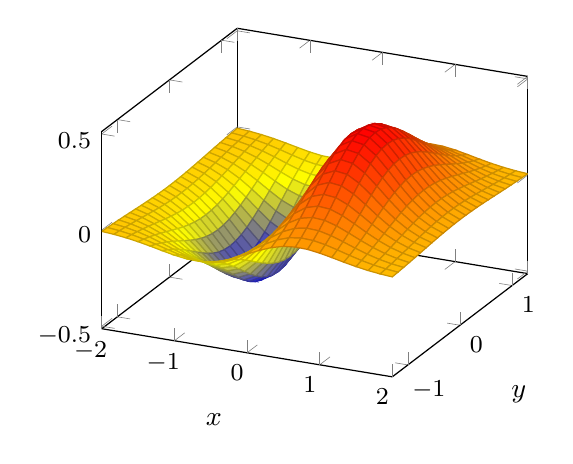
\begin{tikzpicture}[scale=1.1]
	\begin{axis}[
	xlabel=$x$, ylabel=$y$,
	small,
	]
	\addplot3 [
	surf,
	domain=-2:2,
	domain y=-1.3:1.3,
	] {exp(-x^2-y^2)*x};
	\end{axis}
	\end{tikzpicture}
	\caption{$x\cdot \exp(-x^2-y^2)$ 函數圖}
	\label{fig:sig}
\end{figure}
圖\ref{fig:sig}表示$x\cdot \exp(-x^2-y^2)$ 函數圖.



\subsubsection{圖示例:單標題多子圖}
\par 一標題多子圖示例

\tikzstyle{every pin}=[fill=white,draw=black,font=\small,]
\begin{figure}[H]
	\centering
	\begin{subfigure}{.49\textwidth}
	  	\centering
		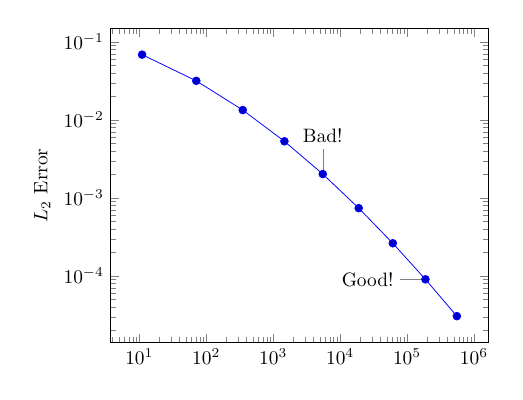
\begin{tikzpicture}[scale=0.7]
			\begin{loglogaxis}[
				%xlabel={\textsc{Dof}},
				ylabel={$L_2$ Error},
				]
				\addplot coordinates {
					(11, 6.887e-02)
					(71, 3.177e-02)
					(351, 1.341e-02)
					(1471, 5.334e-03)
					(5503, 2.027e-03)
					(18943, 7.415e-04)
					(61183, 2.628e-04)
					(187903, 9.063e-05)
					(553983, 3.053e-05)
				};
				\node [coordinate,pin=above:{Bad!}]
				at (axis cs:5503,2.027e-03) {};
				\node [coordinate,pin=left:{Good!}]
				at (axis cs:187903,9.063e-05) {};
			\end{loglogaxis}
		\end{tikzpicture}
		\caption{A subfigure}
		\label{fig:sub1}
	\end{subfigure}
	\begin{subfigure}{.49\textwidth}
		\centering
		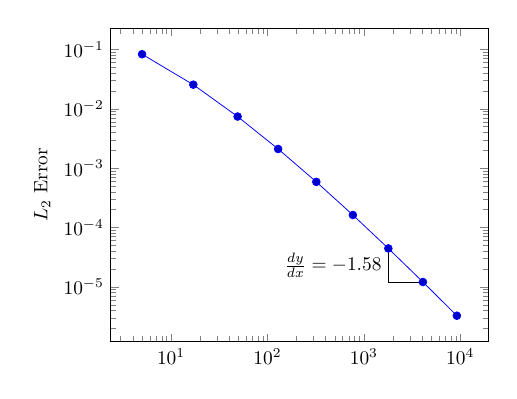
\begin{tikzpicture}[scale=0.7]
			\begin{loglogaxis}[
				ylabel=$L_2$ Error,
				]
				\draw
				(1793,4.442e-05)
				|- (4097,1.207e-05)
				node [near start,left]
				{$\frac{dy}{dx} = -1.58$};
				\addplot coordinates {
					(5, 8.312e-02)
					(17, 2.547e-02)
					(49, 7.407e-03)
					(129, 2.102e-03)
					(321, 5.874e-04)
					(769, 1.623e-04)
					(1793, 4.442e-05)
					(4097, 1.207e-05)
					(9217, 3.261e-06)
				};
			\end{loglogaxis}
		\end{tikzpicture}
		\caption{A subfigure}
	  	\label{fig:sub2}
	\end{subfigure}\\

	\begin{subfigure}{.49\textwidth}
		\centering
		\includegraphics[width=.5\linewidth]{figure/eg05}
		\caption{A subfigure}
		\label{fig:sub3}
	\end{subfigure}
	\begin{subfigure}{.49\textwidth}
		\centering
		\includegraphics[width=.5\linewidth]{figure/eg06}
		\caption{A subfigure}
		\label{fig:sub4}
	\end{subfigure}
	\caption{A figure with two subfigures}
	\label{fig:sub}
\end{figure}
	
	
上面示例中,子圖\ref{fig:sub1}、子圖\ref{fig:sub2}、子圖\ref{fig:sub3}、子圖\ref{fig:sub4}分別表示子圖

	
	
\subsubsection{圖示例:多標題多圖}
\par 多標題多圖示例
\begin{figure}[H]
	\centering
	\begin{minipage}{.48\textwidth}
		\centering

		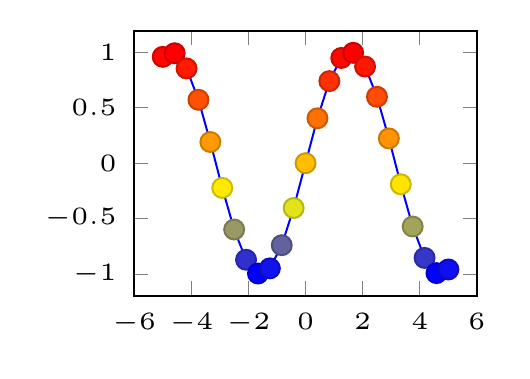
\begin{tikzpicture}[scale=1.8]
		\begin{axis}[tiny]
		\addplot+ [scatter] {sin(deg(x))};
		\end{axis}
		\end{tikzpicture}

		\captionof{figure}{A figure}
		\label{fig:test1}
	\end{minipage}%
	\begin{minipage}{.48\textwidth}
		\centering
		
		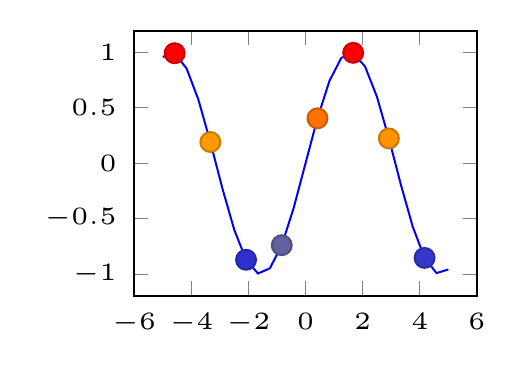
\begin{tikzpicture}[scale=1.8]
		\begin{axis}[tiny]
		\addplot+ [scatter,
		mark repeat=3,mark phase=2]
		{sin(deg(x))};
		\end{axis}
		\end{tikzpicture}
			
		\captionof{figure}{Another figure}
		\label{fig:test2}
	\end{minipage}
\end{figure}
上面示例中,圖\ref{fig:test1}、圖\ref{fig:test2}分別表示兩張獨立的圖


\subsection{示例:表格格式要求}
\par 表:居中,表的標題在表格的上方,編號以“表 2-1”(第二章第一個表)表
示,以後的表按順序排列,表\ref{tab:t1},表 2-2;表 3-1(第三章第一個表)以此類推。


\begin{table}[H]	
	\centering
	\caption{示例正常小表}
	\begin{tabular}[l]{@{}lcccccc}		
		\toprule		
		Class$^{\rm a}$ & $\gamma_1$ & $\gamma_2$$^{\rm b}$& $\langle \gamma \rangle$& $G$ & $|{ f}|$ & $\theta _{c}$ \\		
		\midrule	
		BL Lacs &5 & 36 & 7 & $-4.0$ & $1.0\times 10^{-2}$ & 10$^\circ$ \\		
		FSRQs & 5 & 40 & 11 & $-2.3$ & $0.5\times 10^{-2}$ & 14$^\circ$ \\		
		\bottomrule		
	\end{tabular}
	\label{tab:t1}
\end{table}

下麵是一張超長表
\begin{sidewaystable}[!htp]
	
	\caption{示例旋轉長表} 
	\centering
	\setlength{\tabcolsep}{10mm}
	\begin{tabular}[l]{@{}lcccccc}		
	\toprule		
	Class$^{\rm a}$ & $\gamma_1$ & $\gamma_2$$^{\rm b}$& $\langle \gamma \rangle$& $G$ & $|{ f}|$ & $\theta _{c}$ \\		
	\midrule	
	BL Lacs &5 & 36 & 7 & $-4.0$ & $1.0\times 10^{-2}$ & 10$^\circ$ \\		
	FSRQs & 5 & 40 & 11 & $-2.3$ & $0.5\times 10^{-2}$ & 14$^\circ$ \\		
	\bottomrule		
\end{tabular}
\end{sidewaystable}


$\mathfrak{fer}$















\chapter{結論和建議}
結論由研究結果引伸而來,相同的研究結果,不同的研究者可能引伸
出不同的結果,作者可表達對此結果具有的理論和實際價值的看法。
結論內容碩士一般在 1000 至 2000 字之間,博士一般在 6000 至
10000 字之間,具體要求如下:

(1) 包括研究過程中所遇到或引發的種種現象思考、根據研究成果,提
出解決問題的方向,以及未來值得研究的方向。

(2) 結論要根據論文寫出總結性內容,觀點需具體明確,要有自己的創
見。

(3) 應直接回答研究問題。論據充分,層次清楚,觀點明確,要點分明,
評論合理可信。提示進一步研究的問題,交待本研究是否具體可行,
提示亟待改進之處,詳細地交待研究限制。建議應具參考價值。




%% -------------------------------------------------<< bib 參考文獻 中英文 bib 文件要分别创建
\bibreference



%% -------------------------------------------------<< 附錄
\MUSTappendix{
	
\subsection*{A.1~偽代碼}
\begin{algorithm} 
	\SetAlgoVlined %設置帶水平線的連線
	\caption{identifyRowContext} 
	\KwIn{$r_i$, $Backgrd(T_i)$=${T_1,T_2,\ldots ,T_n}$ and similarity threshold $\theta_r$} 
	\KwOut{$con(r_i)$} 
	$con(r_i)= \Phi$\; 
	\For{$j=1;j \le n;j \ne i$} 
	{ 
		float $maxSim=0$\; 
		$r^{maxSim}=null$\; 
		\While{not end of $T_j$} 
		{ 
			compute Jaro($r_i,r_m$)($r_m\in T_j$)\; 
			\If{$(Jaro(r_i,r_m) \ge \theta_r)\wedge (Jaro(r_i,r_m)\ge r^{maxSim})$} 
			{ 
				replace $r^{maxSim}$ with $r_m$\; 
			} 
		} 
		$con(r_i)=con(r_i)\cup {r^{maxSim}}$\; 
	} 
	return $con(r_i)$\; 
\end{algorithm}


\subsection*{A.2~smithchart mirrored}
\begin{figure}[H]
	\centering
	\begin{tikzpicture}[scale=1.2]
	\begin{smithchart}[smithchart mirrored,]
	\addplot coordinates {
		(0.5,0.2) (1,0.8) (2,2)
	};
	\end{smithchart}
	\end{tikzpicture}
	
\end{figure}














\subsection*{A.3~plot3D}
\begin{figure}[H]

	\begin{subfigure}{.49\textwidth}
		\centering
		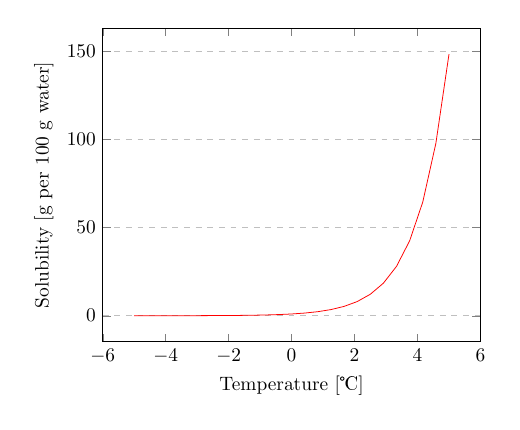
\begin{tikzpicture}[scale=0.7]
		\begin{axis}[
		xlabel={Temperature [\textcelsius]},
		ylabel={Solubility [g per 100 g water]},
		ymajorgrids=true,
		grid style=dashed,]
		\addplot[color=red]{exp(x)};
		\end{axis}
		\end{tikzpicture}
		\caption{A subfigure}
	\end{subfigure}
%-----------------------------------------------------------
	\begin{subfigure}{.49\textwidth}
		\centering
		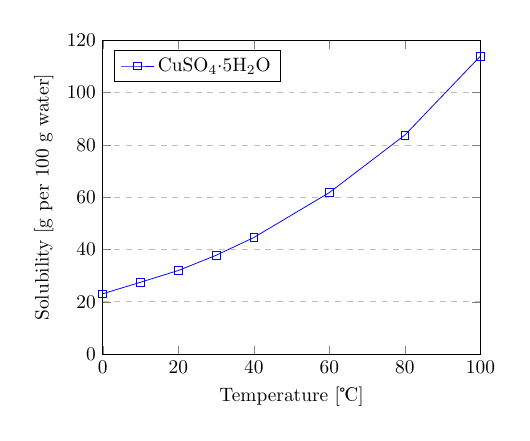
\begin{tikzpicture}[scale=.7]
			\begin{axis}[
				xlabel={Temperature [\textcelsius]},
				ylabel={Solubility [g per 100 g water]},
				xmin=0, xmax=100,
				ymin=0, ymax=120,
				xtick={0,20,40,60,80,100},
				ytick={0,20,40,60,80,100,120},
				legend pos=north west,
				ymajorgrids=true,
				grid style=dashed,
				]
				\addplot[
				color=blue,
				mark=square,
				]
				coordinates {
					(0,23.1)(10,27.5)(20,32)(30,37.8)(40,44.6)(60,61.8)(80,83.8)(100,114)
				};
				\legend{CuSO$_4\cdot$5H$_2$O}
			\end{axis}
		\end{tikzpicture}
		\caption{A subfigure}
	\end{subfigure}
%-----------------------------------------------------------
	\centering
	\begin{subfigure}{.49\textwidth}
		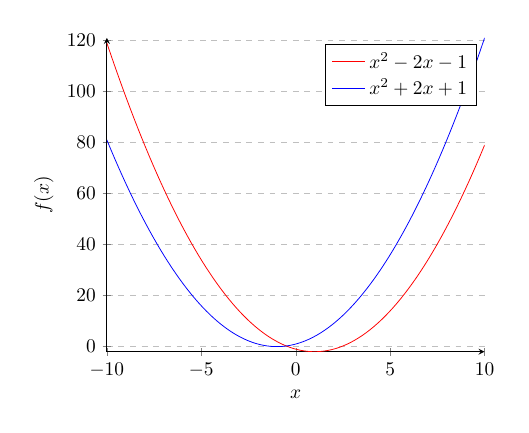
\begin{tikzpicture}[scale=0.7]
			\begin{axis}[
				axis lines = left,
				xlabel = $x$,
				ylabel = {$f(x)$},
				ymajorgrids=true,
				grid style=dashed,]
				]
				%Below the red parabola is defined
				\addplot [
				domain=-10:10, 
				samples=100, 
				color=red,
				]
				{x^2 - 2*x - 1};
				\addlegendentry{$x^2 - 2x - 1$}
				%Here the blue parabloa is defined
				\addplot [
				domain=-10:10, 
				samples=100, 
				color=blue,
				]
				{x^2 + 2*x + 1};
				\addlegendentry{$x^2 + 2x + 1$}
			\end{axis}
		\end{tikzpicture}
		\caption{A subfigure}
	\end{subfigure}
\end{figure}




\subsection*{A.4~plot3D}
\begin{figure}[H]
	\centering
	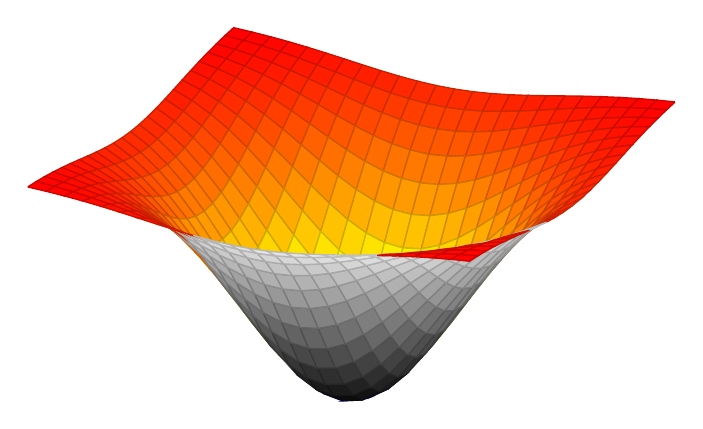
\begin{tikzpicture}[scale=1.2]
	\begin{axis}[
	hide axis,
	xlabel=$x$,ylabel=$y$,
	mesh/interior colormap name=hot,
	colormap/blackwhite,
	]
	\addplot3 [domain=-1.5:1.5,surf]
	{-exp(-x^2-y^2)};
	\end{axis}
	\end{tikzpicture}

app:plot3D
\end{figure}
}


%% -------------------------------------------------<< 致謝
\MUSTacknowledgement{
	一路過來,感恩所有人!
}















%% -------------------------------------------------<< 個人簡歷
% 入學時間
\def\mustProfilea{
	2019年5月10日
}


% 起止年月
\def\mustProfileb{
	2010.11 $\sim$ 2011.11 \\
	2010.11 $\sim$ 2011.11
}


% 就讀學校
\def\mustProfilec{
	X~X~X~大學 \\
	X~X~X~大學
}


% 取得學位名稱
\def\mustProfiled{
	X~X~学士学位\\
	X~X~硕士学位
}


%發表的學術論文、著作(論文/著作名稱、報刊/出版社名稱、發表時間、刊物/出版社級別)
\def\mustProfilee{
	待写,待补
}


%參加的學術項目(項目名稱、項目時間、立項單位、承擔的工作)
\def\mustProfilef{
	待写,待补
}



% 自动生成個人簡歷
\MUSTProfile



\end{document}
